\documentclass[twocolumn]{article}

%% Language and font encodings
\usepackage[english]{babel}
\usepackage[utf8]{inputenc}
\usepackage{csquotes}
\bibliographystyle{unsrt}
\usepackage{booktabs}

\usepackage{tabu}
\usepackage[T1]{fontenc}

%% Sets page size and margins
\usepackage[a4paper,top=2cm,bottom=2cm,left=3cm,right=3cm,marginparwidth=1.75cm]{geometry}

%% Useful packages
\usepackage{amsmath}
\usepackage{graphicx}
%\usepackage{apacite}
\usepackage[colorinlistoftodos]{todonotes}
\usepackage[colorlinks=true, allcolors=blue]{hyperref}

\title {{\it Project-} Automated Handwritten Digit Recognition Using Machine Learning}
\author{B. Shadrack Jabes}
\date{\it{\today}}

\begin{document}
\maketitle

\section{Introduction}
The aim of this project is to write a backprobagation algorithm for neural networks and predict the handwritten digits. 
\section{Dataset}
Each handwritten alphabet is a 20 pixel by 20 pixel grayscale image. One can view the pixels as floating point numbers indicating the intensity of the gray scale at a particular location. I then unrol the 20 x 20 pixel into a a single row of 400 dimensional vector. There are 5000 such handwritten images. Therefore a total of 5000 x 400 handwritten digit images should be handled.
	   \begin{figure}[htbp]
                \centering
                \includegraphics[clip=true,trim=0cm 0cm 0cm 0cm,width=8cm]{../dataset.ps}
                        \caption{Handwritten digit image. Randomly seleted 100 digits are shown here. Each digit shown here is a 20 pixel by 20 pixel image.}
                \label{fig:dataset}
                \end{figure}
\section{Artificial neural network model}
The model consists of three layers: input layer with 400 units each corresponding to the pixel description of one digit, hidden layer with 25 units and a output layer with 10 units. The 10 units in the outputlayer corresponds to the 10 total labels the digits belong to. That is a widely used handwritten digit image from zero to nine. The digit 'zero' is mapped to label '10', while the other digits are labelled in naturally. For instance when the image 6 is selected, then the corresponding $y^{(i)}$ that must be used in the cost function (described below) should be a 10 dimensional vector with $y_5 = 1$, and the other elements are set to zero.
	   \begin{figure}[htbp]
                \centering
                \includegraphics[clip=true,trim=0cm 0cm 0cm 0cm,width=8cm]{../ann.ps}
                        \caption{Neural network model.}
                \label{fig:ann}
                \end{figure}
\section{Feedforward propagation and cost}

\subsection{Input layer}
$x$ is the input layer of shape (m,1), where $m$ is the number of input neurons.
\begin{align*}
	x = [x_1, x_2 ....x_m]
\end{align*}
\subsection{Bias}
$b$ is the bias vector. This is an extra unit with a value of $+1$ in each layer except the output layer.
\subsection{Weights or $\Theta$}
$\theta(l)$ is a weight matrix of shape (n,m), where $n$ is the number of neurons in the next layer and $m$ is the neurons in the previous layer.
\subsection{Neuron value Z$^l$ and activation value a$^l$}
The value of $Z^l$ of each neuron in each layer $l$ is given as follows
\begin{align*}
	z^{(2)} = [\theta_{11}^{(1)}a_1 + . . .\theta_{1,m}^{(1)}a_1 + b_1^{(1)} ;\\... \theta_{n,1}^{(1)}a_1 + . . .\theta_{n,m}^{(1)}a_1 + b_n^{(1)}]
\end{align*}
\begin{align*}
	a^{(2)} = g(z^{(2)}) = \frac{1}{1 + e^{-z^{(2)}}}\\
	h_{\theta}(x^{(2)}) = a^{(2)}
\end{align*}
\subsection{Cost}
Then I compute the cost function for the neural network as described here
\begin{align*}
	J(\theta) =\\ \frac{1}{m}\sum_{i=1}^m\sum_{k=1}^K [-y_k^{(i)} log((h_{\theta}(x^{(i)}))_k)]\\ - [(1-y_k^{(i)}) log(1-(h_{\theta}(x^{(i)}))_k))]\\ + \frac{\lambda}{2m}[\sum_{j=1}^{25}\sum_{k=1}^{400}(\theta_{j,k}^{(1)})^2 \\ + \sum_{j=1}^{10}\sum_{k=1}^{25}(\theta_{j,k}^{(2)})^2]
\end{align*}
Here for instance $h_{\theta}(x^{(i)}) = a_k^{(3)}$, is the activation or output value of the k$^{th}$  unit of the third layer. A total of $K = 10$ labels are considered in this example. To minimize the cost I have to adjust the parameters in an orderly fashion. This is done using the following backpropagation algorithm.
\section{Backpropagation}
The idea is to compute the activations (i.e.,) $h_{\theta}(x^{(i)})$ using forward approach but compute the error using back propagation.
The parameters corresponding to the minimum cost can be obtained by looking at the gradient of the cost function. To compute the gradient of the cost function I perform backpropagation which I discuss here.
For each node in layer $l$ , I noe compute an 'error term'  that measures how much that node was 'responsible' for any errors in our output.
\begin{align*}
	g'(z) = \frac{dg(z)}{dz} = g(z)(1-g(z))\\
	g(z) =  \frac{1}{1+e^-z}
\end{align*}
From the output node I compute the error ($\delta$) to be the difference between the activation unit ($a$) and target value ($y$), $\delta_j^{(3)} = a_j^{(3)} - y_j$. The error in the hidden units are computed as follows:
\begin{align*}
	\delta^{(2)} = (\theta^{(2)})^T\delta^{(3)}.*g'(z^{(2)})\\
	\Delta{(l)} = \Delta{(l)} + \delta{(l+1)}(a{(l)})^T\\
	\frac{dJ(\theta)}{d\theta_{ij}^{(l)}} = \frac{1}{m}\Delta_{ij}^{(l)}
\end{align*}
\section{Contribution}
I have implemented the vectorized backpropagation neural network code in this project.
\end{document}
